\chapter{Estado de la Cuestión}
\label{cap:estadoDeLaCuestion}
Este capítulo muestra la perspectiva teórica de la investigación llevada a cabo como trabajo previo al desarrollo del código. El conocimiento que se presenta en las siguientes páginas es necesario para entender cuál era el contexto del problema y el porqué de las decisiones que se han tomado para la construcción de la solución.

La estructura del capítulo muestra, en orden temporal, las herramientas del procesamiento de lenguaje que se han ido popularizando, desde las alternativas históricas hasta la situación actual. De está forma, nos permite entender su importancia y conocer otras alternativas de implementación.

Finalmente, este capítulo muestra trabajos relacionados, ya sean puntos de partida para el trabajo actual, trabajos que complementan al presente proyecto, o incluso otros trabajos que cuyo estudio ha servido como herramienta de aprendizaje de cara a preparar el $chatbot$. 

En conclusión, se pretende dar una perspectiva global de la situación actual en la que se encuentra el procesamiento del lenguaje en general y el desarrollo del $chatbot$ en particular.  
\newpage
\section{Evolución del Procesamiento del Lenguaje Natural}
El procesamiento del lenguaje natural (PLN) ha experimentado una evolución notable, impulsada por avances tecnológicos como la inteligencia artificial (IA). La integración de técnicas de IA en el PLN dió lugar a la rama del procesamiento natural del lenguaje (PLN), que supuso todo un hito en el ámbito del lenguaje escrito.

Inicialmente, los algoritmos de PLN se basaban en reglas, pero con el tiempo se adoptaron modelos de clasificación supervisada. Sin embargo, estos modelos enfrentaban limitaciones al no capturar el contexto completo de las palabras en una frase. Tres avances clave marcaron el camino hacia una PNL más avanzada. 

Primero, el surgimiendo de los modelos $word$ $embeddings$ descritos en la sección \ref{sec:WordEmbeddings}, desarrollados en 2013 que permiten representar palabras en un espacio vectorial considerando su contexto, lo que facilita la comprensión de sinónimos y relaciones entre palabras. 

En segundo lugar, la arquitectura de redes neuronales profundas conocida como $transformers$, descritos en la sección \ref{sec:Transformers}, revolucionó el campo al capturar el contexto completo de un texto mediante una matriz de atención. Además, los modelos basados en $transformers$ permiten la transferencia de aprendizaje, lo que facilita la adaptación a diversas aplicaciones.

Finalmente, el surgimiento de modelos generativos de lenguaje multipropósito de gran tamaño, como el archiconocido ChatGPT, ha llevado la PNL a nuevos horizontes. Estos modelos, que se describen en la sección \ref{sec:LLM} con cientos de millones de parámetros, pueden generar texto de calidad comparable a la humana y están generando debates sobre su impacto en diversos ámbitos. 

A pesar de estos avances, persisten desafíos en el PLN, como la necesidad de bases de datos específicas y validadas para el entrenamiento de modelos especializados. Los investigadores son llamados a trabajar en la construcción de nuevas bases de datos y en el desarrollo de esquemas de preprocesamiento y ajuste, con el objetivo de impulsar soluciones a problemas específicos a nivel global.

\section{Word embeddings}
\label{sec:WordEmbeddings}

Los $word$ $embeddings$ \citep{wordEmbeddings} son una técnica importante en el procesamiento del lenguaje natural que consiste en representar palabras y documentos como vectores numéricos en un espacio de dimensiones reales. Este enfoque permite que palabras con significados similares tengan representaciones vectoriales similares, lo que facilita que las computadoras comprendan el contenido basado en texto de manera más efectiva.

En los $word$ $embeddings$, las palabras se representan como vectores numéricos en un espacio dimensional reducido, lo que permite capturar información semántica y sintáctica entre palabras. Estos vectores se utilizan como características para alimentar modelos de aprendizaje automático, lo que permite trabajar con datos de texto y preservar la información semántica y sintáctica. Existen diferentes técnicas para tratar los $word$ $embeddings$.

\subsection{TF-IDF}

La frecuencia de término-inversa de frecuencia de documento (TF-IDF) es un algoritmo de aprendizaje automático que se utiliza para la incrustación de palabras en texto. Consta de dos métricas: frecuencia de término (TF) y la inversa de la frecuencia de documento (IDF).

Este algoritmo trabaja en una medida estadística para encontrar la relevancia de las palabras en el texto, que puede estar en forma de un solo documento o varios documentos referidos como corpus.

\begin{center}
$\textbf{tf-idf}_{i,j} =$ Frecuencia del término $i$ en el documento $j$ $\times$ Frecuencia inversa de documentos del término $i$
\end{center}

El puntaje de frecuencia de término (TF) mide la frecuencia de las palabras en un documento particular. En otras palabras, cuenta la ocurrencia de palabras en los documentos.
\begin{center}
	$\textbf{tf}_{i,j} =  \frac{\textit{Frecuencia del término } i \textit{ en el documento } j}{\textit{Número total de términos en } j}$ 
\end{center}


La inversa de la frecuencia de documento (IDF) mide la rareza de las palabras en el texto. Se le otorga más importancia que el puntaje de frecuencia de término porque, aunque el puntaje de TF otorga más peso a las palabras que ocurren con frecuencia, el puntaje de IDF se centra en las palabras raramente utilizadas en el corpus que pueden contener información significativa.
\begin{center}
	$\textbf{idf}_{i} = \log \left( \frac{\textit{Número total de documentos}}{\textit{Número de documentos que contienen el término } i} \right)$
\end{center}


El algoritmo TF-IDF se utiliza en tareas básicas de procesamiento de lenguaje natural y aprendizaje automático, como la recuperación de información, eliminación de palabras vacías, extracción de palabras clave y análisis de texto. Sin embargo, no captura eficientemente el significado semántico de las palabras en una secuencia.

\subsection{Bolsa de palabras}
	
El Bag of Words (BoW) es una técnica de procesamiento de texto ampliamente utilizada en el procesamiento del lenguaje natural (PLN) y la minería de texto. Esta técnica consiste en representar un documento de texto como un conjunto de palabras, ignorando el orden y la estructura gramatical.
	
En el modelo BoW, se crea un vocabulario de todas las palabras únicas en un conjunto de documentos de texto. Cada documento se representa como un vector de tamaño igual al tamaño del vocabulario, donde cada posición en el vector indica la frecuencia de una palabra en el documento.
	
Por ejemplo, si el vocabulario contiene las palabras "gato", "perro" y "juguete", y un documento tiene una frecuencia de dos para "gato" y tres para "perro", su vector de representación BoW sería [2,3,0].
	
La técnica BoW es útil para la clasificación y agrupación de documentos basados en su contenido textual. Se utiliza en aplicaciones como análisis de sentimientos, clasificación de texto y recomendación de contenidos.
	
El proceso de creación de la matriz BoW se lleva a cabo en varios pasos:
\begin{enumerate}
	\item \textbf{Creación del vocabulario}: Se genera un conjunto de palabras únicas a partir de todos los documentos de texto.
	\item \textbf{Vectorización del texto}: Cada documento se convierte en un vector de tamaño igual al vocabulario, donde las palabras presentes en el documento tienen un valor de uno, y las ausentes tienen un valor de cero.
	\item \textbf{Normalización del peso}: Los vectores se normalizan dividiendo cada valor por la suma total de valores en el vector.
\end{enumerate}

Una vez creada la matriz BoW, se puede utilizar en diversas aplicaciones de inteligencia artificial, como la clasificación de textos, el análisis de sentimientos y la agrupación de documentos.


\subsection{Word2Vec}
El método Word2Vec, desarrollado por Google en 2013, revolucionó el campo del procesamiento del lenguaje natural (PLN) al ofrecer una forma innovadora de entrenar incrustaciones de palabras. Este enfoque se basa en una idea distributiva que utiliza skip-grams o una técnica llamada Bolsa Continua de Palabras (CBOW).

En esencia, Word2Vec emplea redes neuronales poco profundas con capas de entrada, salida y proyección. Estas redes tienen como objetivo reconstruir el contexto lingüístico de las palabras, considerando tanto su orden en el texto como su contexto futuro.

El proceso implica iterar sobre un corpus de texto para aprender las asociaciones entre palabras. Se fundamenta en la premisa de que las palabras que aparecen juntas en un texto tienen una similitud semántica entre ellas. Esto permite asignar representaciones vectoriales a las palabras que son cercanas geométricamente en el espacio vectorial.

La similitud del coseno se utiliza como métrica para medir cuán similares son dos palabras o documentos en su significado. Si el ángulo entre los vectores de palabras es pequeño, la similitud del coseno es alta, lo que indica que las palabras tienen significados similares. Por el contrario, si el ángulo es de 90 grados, la similitud es baja, lo que indica que las palabras son independientes en su contexto.

\section{Transformers}
\label{sec:Transformers}

Los modelos pre-entrenados son modelos de aprendizaje profundo o $Deep Learning$ que sirven para realizar diversas tareas de Procesamiento de Lenguaje. Son pre-entrenados bajo grandes conjuntos de datos, lo que les permite ajustarse a atareas específicas sin requerir un entrenamiento desde cero. Este pre-entrenamiento es clave para entender por qué son tan valiosos, ya que permiten construir un sistema de generación de lenguaje sin un gran esfuerzo computacional (normalmente los entrenamientos tardan semanas o meses incluso con los mejores computadores). 

Dentro de los modelos pre-entrenados, toman especial importancia los $transformers$ (\cite{transformers}). Desde el primer momento, revolucionaron el PLN al introducir mecanismos de atención auto-ajustable, paralelización eficiente, captura de contexto bidireccional y pre-entrenamiento masivo. Todo ello permite construir modelos más poderosos y efectivos. 

\subsection{Aprendizaje por transferencia}
Los modelos pre-entrenados, frente a los modelos estadísticos u otros tipos de algoritmos de \textit{Deep Learning}, suponen grandes ventajas debido al pre-entrenamiento bajo un gran conjunto de datos y un pequeño ajuste posterior a realizar para adaptarlo a la tarea que se desee resolver, exigiendo mucho menos coste computacional y requiriendo para ello menos tiempo y esfuerzo. Todo esto es posible gracias al aprendizaje por transferencia o \textit{Transfer Learning}.

El \textit{Transfer Learning} es fundamental en el desarrollo y la eficiencia de los modelos pre-entrenados. Aparecen como solución al paradigma del aprendizaje aislado que presentan algoritmos como el aprendizaje supervisado tradicional. Estos modelos pueden aprovechar el conocimiento adquirido previamente en grandes conjuntos de datos para adaptarse a nuevas tareas con un costo computacional y de tiempo significativamente menor que si se entrenaran desde cero. Este enfoque es especialmente valioso en campos como la visión artificial o el PLN.

En el ámbito de la visión artificial, los modelos pre-entrenados pueden ser adaptados para tareas específicas, como la clasificación de imágenes, mediante el aprendizaje por transferencia. Por ejemplo en \cite{tu2018transfer}, el sistema utiliza redes neuronales convolucionales pre-entrenadas para reconocer perros en imágenes, aprovechando el conocimiento previo adquirido por el modelo.

En PLN, los modelos pre-entrenados también son esenciales para resolver diversas tareas, como la detección de noticias falsas (\cite{slovikovskaya2019transfer}). Estos modelos pueden emplear el aprendizaje por transferencia para adaptarse a nuevas tareas, como la clasificación de texto, utilizando el conocimiento previo obtenido durante el entrenamiento inicial.

Dentro del aprendizaje por transferencia, existen varias técnicas, como la adaptación de dominio, la confusión de dominio, el aprendizaje de una sola muestra ($One-shot Learning$), el aprendizaje de cero muestras ($Zero-shot Learning$) y el aprendizaje multitarea. Este último, utilizado por modelos como T5, tiene como objetivo crear modelos generalistas capaces de resolver múltiples tareas, en contraposición a modelos especializados en una sola tarea.

\section{Modelos de Lenguaje de Gran Tamaño (LLM)}
\label{sec:LLM}

La invención de los transformadores marcó el comienzo de la era de los grandes modelos de lenguaje modernos. Desde 2018, los laboratorios de IA han comenzado a entrenar modelos cada vez más grandes, conocidos como LLM.
	
Los Modelos de Lenguaje de Gran Tamaño (LLM) son modelos de aprendizaje profundo que se entrenan con grandes cantidades de datos utilizando la arquitectura de transformadores. Estos modelos constan de un codificador y un decodificador que trabajan en conjunto para entender y generar texto. 

Hay tres lineas de desarrollo principales para estos modelos de lenguaje, y múltitud de modelos como se puee ver en la figura \ref{fig:3.1}. 

\begin{figure}[h]
	\centering
	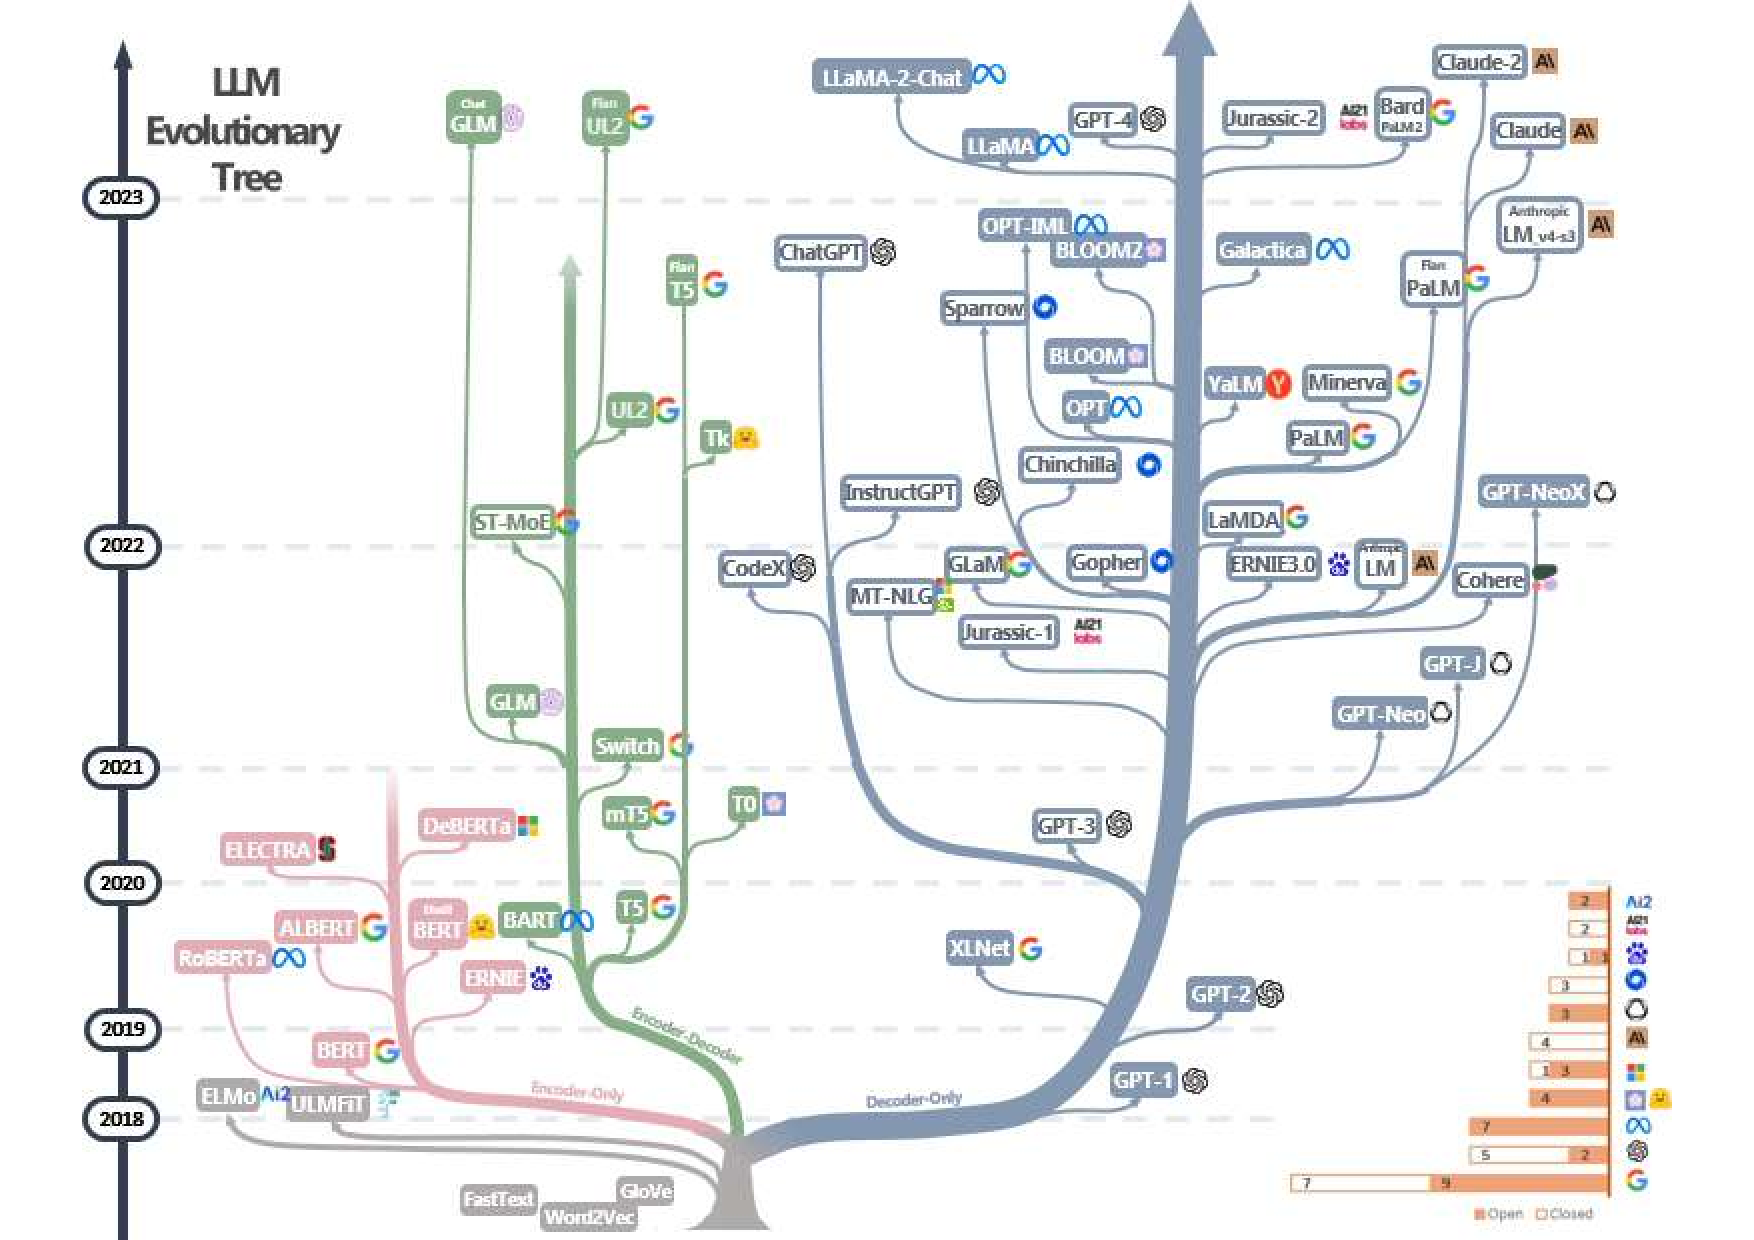
\includegraphics[width=1\textwidth]{Imagenes/treeLLM}
	\caption{Desarrollo de los LLM por\cite{yang2023harnessing}}
	\label{fig:3.1}
\end{figure}

Por un lado, el grupo ``solo codificador'', mostrado en rosa en la figura \ref{fig:3.1} incluye LLM que son buenos para la comprensión del texto porque permiten que la información fluya en ambas direcciones del texto. En azul, podemos ver el grupo ``solo decodificador'' que incluye LLM que son buenos en la generación de texto porque la información solo fluye de izquierda a derecha del texto para generar nuevas palabras de manera eficiente y autorregresiva. Finalmente, hay un tipo codificador-decodificador (mostrado en verde) que combina ambos aspectos y se usa para tareas que requieren comprender una entrada y generar una salida, como la traducción. 

Dentro de este último grupo encontramos la mayoría de los modelos que fueron considerados para el desarrollo de este trabajo como los distintos modelos de GPT, los de Google (Bard, que evolucionó a Gemini, LaMDA o PaLM).
\subsection{BERT}
Los modelos de lenguaje enmascarados, como los Masked Language Models, enmascaran un cierto porcentaje de palabras en una oración y se espera que el modelo prediga esas palabras en función del contexto restante \cite{rothman2022}. Un ejemplo representativo de este enfoque es BERT.

BERT (\textit{Bidirectional Encoder Representations from Transformers}) es un modelo de lenguaje enmascarado basado en la arquitectura Transformer \cite{devlin2019bert}. Desarrollado por Google en 2018, BERT ha demostrado un rendimiento sobresaliente en una variedad de tareas de procesamiento de lenguaje natural.

BERT se pre-entrena en dos grandes corpus de texto en inglés sin etiquetar: BookCorpus \cite{zhu2015aligning} y Wikipedia. Estos corpus garantizan una amplia cobertura de datos y una buena calidad para el entrenamiento del modelo.

Aunque inicialmente no estaba diseñado para la generación de texto, BERT ha sido adaptado para esta tarea, logrando mejoras significativas en comparación con modelos como GPT-2 \cite{wang2019bert}.

Existen numerosas variantes de BERT, algunas pre-entrenadas en dominios específicos y otras con un ajuste fino para tareas específicas \cite{rajasekharan2019review}. Por ejemplo, Beto es la versión en español de BERT, entrenada en un corpus extenso en dicho idioma \cite{canete2020spanish}.

La innovación clave de BERT es su enfoque bidireccional, que permite al modelo comprender el contexto de una palabra en función de su entorno completo. A diferencia de modelos unidireccionales como GPT-2, BERT considera tanto el contexto anterior como el posterior a una palabra dada.

La arquitectura de BERT consiste en una pila de codificadores de transformadores, con un número variable de capas dependiendo de la versión del modelo. Este enfoque permite a BERT realizar múltiples tareas de procesamiento de lenguaje, incluyendo Modelado de Lenguaje Enmascarado y Predicción de la Siguiente Oración \cite{devlin2019bert}.		


\subsection{T5}

T5, o Text-to-Text Transfer Transformer \cite{T5}, es un marco unificado para el aprendizaje por transferencia en procesamiento de lenguaje natural (PLN). Este enfoque revolucionario convierte todos los problemas basados en texto en un formato de texto a texto, donde el modelo recibe texto como entrada y genera nuevo texto como salida. Inspirado en marcos anteriores para tareas de NLP, como la modelización de lenguaje o la extracción de fragmentos, T5 permite aplicar el mismo modelo, objetivo de entrenamiento, procedimiento de entrenamiento y proceso de decodificación a cada tarea considerada.

El objetivo principal de T5 es proporcionar una perspectiva exhaustiva sobre el estado actual del campo de la transferencia de aprendizaje para PLN. En lugar de proponer nuevos métodos, se enfoca en la exploración y comparación empírica de técnicas existentes. Además, para facilitar futuros trabajos en este campo, se liberan conjuntos de datos, modelos pre-entrenados y código fuente.

\begin{figure}[h]
	\centering
	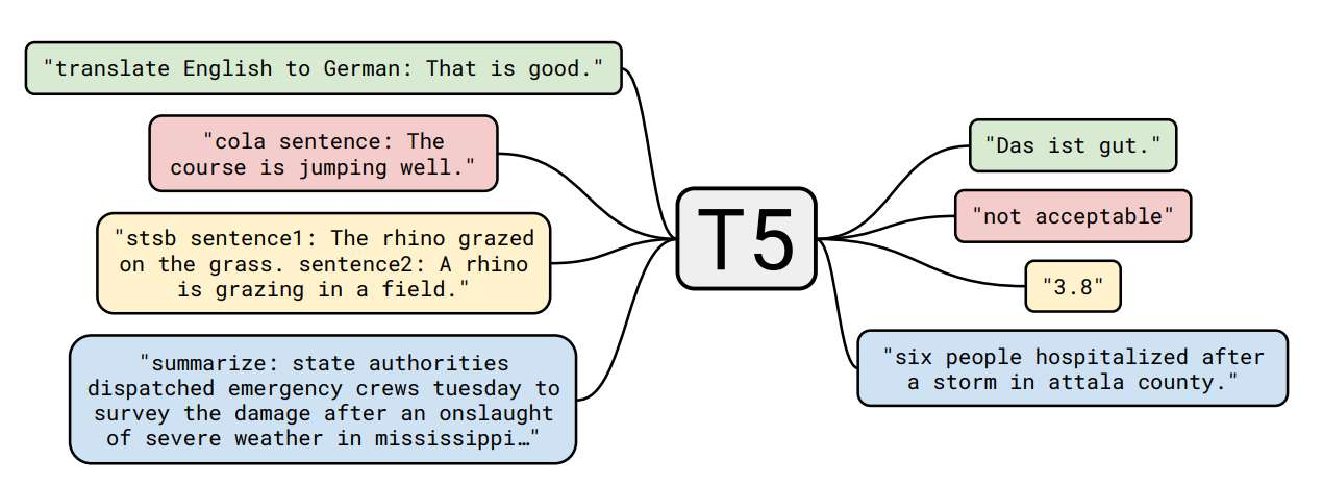
\includegraphics[width=0.9\textwidth]{Imagenes/T5}
	\caption{Diagrama del modelo T5 de \cite{T5}}
	\label{fig:3.2}
\end{figure}

Cómo se puede ver en la figura \ref{fig:3.2} el modelo T5 nos permite realizar diversas tareas como la traducción o la realización de resumenes.
%completar con las otras tareas que nos permite hacer no identifico que hace en lo rojo y amarillo 

\subsection{GPT \textit{Generative Pretrained Transformer}}

Los modelos de lenguaje casual o \textit{Casual Language Models}, tienen como idea principal predecir una palabra o token enmascarado en una oración. Podemos ver una palabra enmascarada como un hueco en blanco en una frase. En este caso, el modelo solo consideraría el contexto anterior (palabras situadas a su izquierda) y dejaría de tener en cuenta el contexto posterior. El sentido de procesamiento (izquierda a derecha o derecha a izquierda) no es relevante mientras que se realice en un único sentido, teniendo en cuenta para la predicción las palabras pertenecientes a ese contexto y dejando de lado el resto de palabras. Así, la propiedad clave de este tipo de modelos es la naturaleza unidireccional en su predicción de las palabras enmascaradas y se verá reflejado en el esquema de entrenamiento \citep{rothman2022}.

\subsubsection{GPT-1}
\textit{Generative Pre-trained Transformer 1}(GPT-1) fue el primer modelo de lenguaje grande de OpenAI siguiendo la invención de la arquitectura transformer por parte de Google en 2017. En junio de 2018, OpenAI publicó un artículo titulado ``Improving Language Understanding by Generative Pre-Training'' \cite{radford2018improving}, en el cual presentaron ese modelo inicial junto con el concepto general de un $transformer$ generativo pre-entrenado.

Hasta ese momento, los modelos neuronales de PLN con mejor rendimiento empleaban principalmente el aprendizaje supervisado a partir de grandes cantidades de datos etiquetados manualmente. Esta dependencia del aprendizaje supervisado limitaba su uso de conjuntos de datos que no estaban bien etiquetados, además de hacer que fuera prohibitivamente costoso y lento entrenar modelos extremadamente grandes; muchos idiomas (como el suajili o el criollo haitiano) son difíciles de traducir e interpretar utilizando tales modelos debido a la falta de texto disponible para la construcción de corpus. En contraste, el enfoque ``semi-supervisado'' de un GPT involucraba dos etapas: una etapa de pre-entrenamiento generativo no supervisado en la que se utilizaba un objetivo de modelado de lenguaje para establecer parámetros iniciales, y una etapa de ajuste fino discriminatorio supervisado en la que estos parámetros se adaptaban a una tarea objetivo.

El uso de una arquitectura transformer, en lugar de técnicas anteriores que involucraban RNNs con atención aumentada, proporcionó a los modelos GPT una memoria más estructurada de lo que se podría lograr a través de mecanismos recurrentes; esto resultó en un robusto rendimiento de transferencia en diversas tareas.

\subsubsection{GPT-2}

GPT-2 es uno de los modelos más representativos de los modelos de lenguaje casual que sigue una arquitectura de tipo Transformer basada en auto-atención (masked self-attention). Presentado por OpenAI en 2019, desde el primer momento fue considerado un gran éxito en el campo del Procesamiento de Lenguaje debido a sus más de 1.5 billones (americanos) de parámetros.

El objetivo de este sistema es construir una distribución de probabilidad en la que para cada palabra posible a generar se le asigna una probabilidad en función del contexto anterior. Este modelo fue pre-entrenado sobre un gran corpus de texto inglés siguiendo el entrenamiento auto-supervisado (self-supervised). El objetivo de este modelo es la predicción de la palabra siguiente dada una secuencia de palabras u oración.

Para pre-entrenar el modelo se creó un conjunto de datos, llamada WebText, formada a partir de la extracción de millones de páginas web obtenidas de enlaces de salida de páginas de Reddit que habían recibido una determinada puntuación mínima (para garantizar la calidad y significancia del enlace). Las páginas de Wikipedia relacionadas con estos enlaces se eliminaron. Es por esto por lo que GPT-2 no está entrenado bajo ningún texto de Wikipedia. El conjunto de datos resultante es un enorme corpus de 40GB de textos preparado para el entrenamiento de este modelo, GPT-2 \cite{radford2019language}.

La estructura de GPT-2 se asemeja mucho a la del modelo Transformer. Originalmente, este modelo constaba de un codificador y un decodificador, diseñado especialmente para tareas específicas como la traducción automática. Sin embargo, GPT-2 abandonó esta arquitectura convencional y optó por utilizar exclusivamente una serie de decodificadores del modelo Transformer. El número de decodificadores utilizados varía según el tamaño de GPT-2: la versión Small emplea solo doce, mientras que la versión Extra Large puede llegar a utilizar hasta cuarenta y ocho decodificadores. Esta configuración basada únicamente en decodificadores, característica distintiva de GPT-2, se ilustra en la figura 2.17.

\begin{figure}[h]
	\centering
	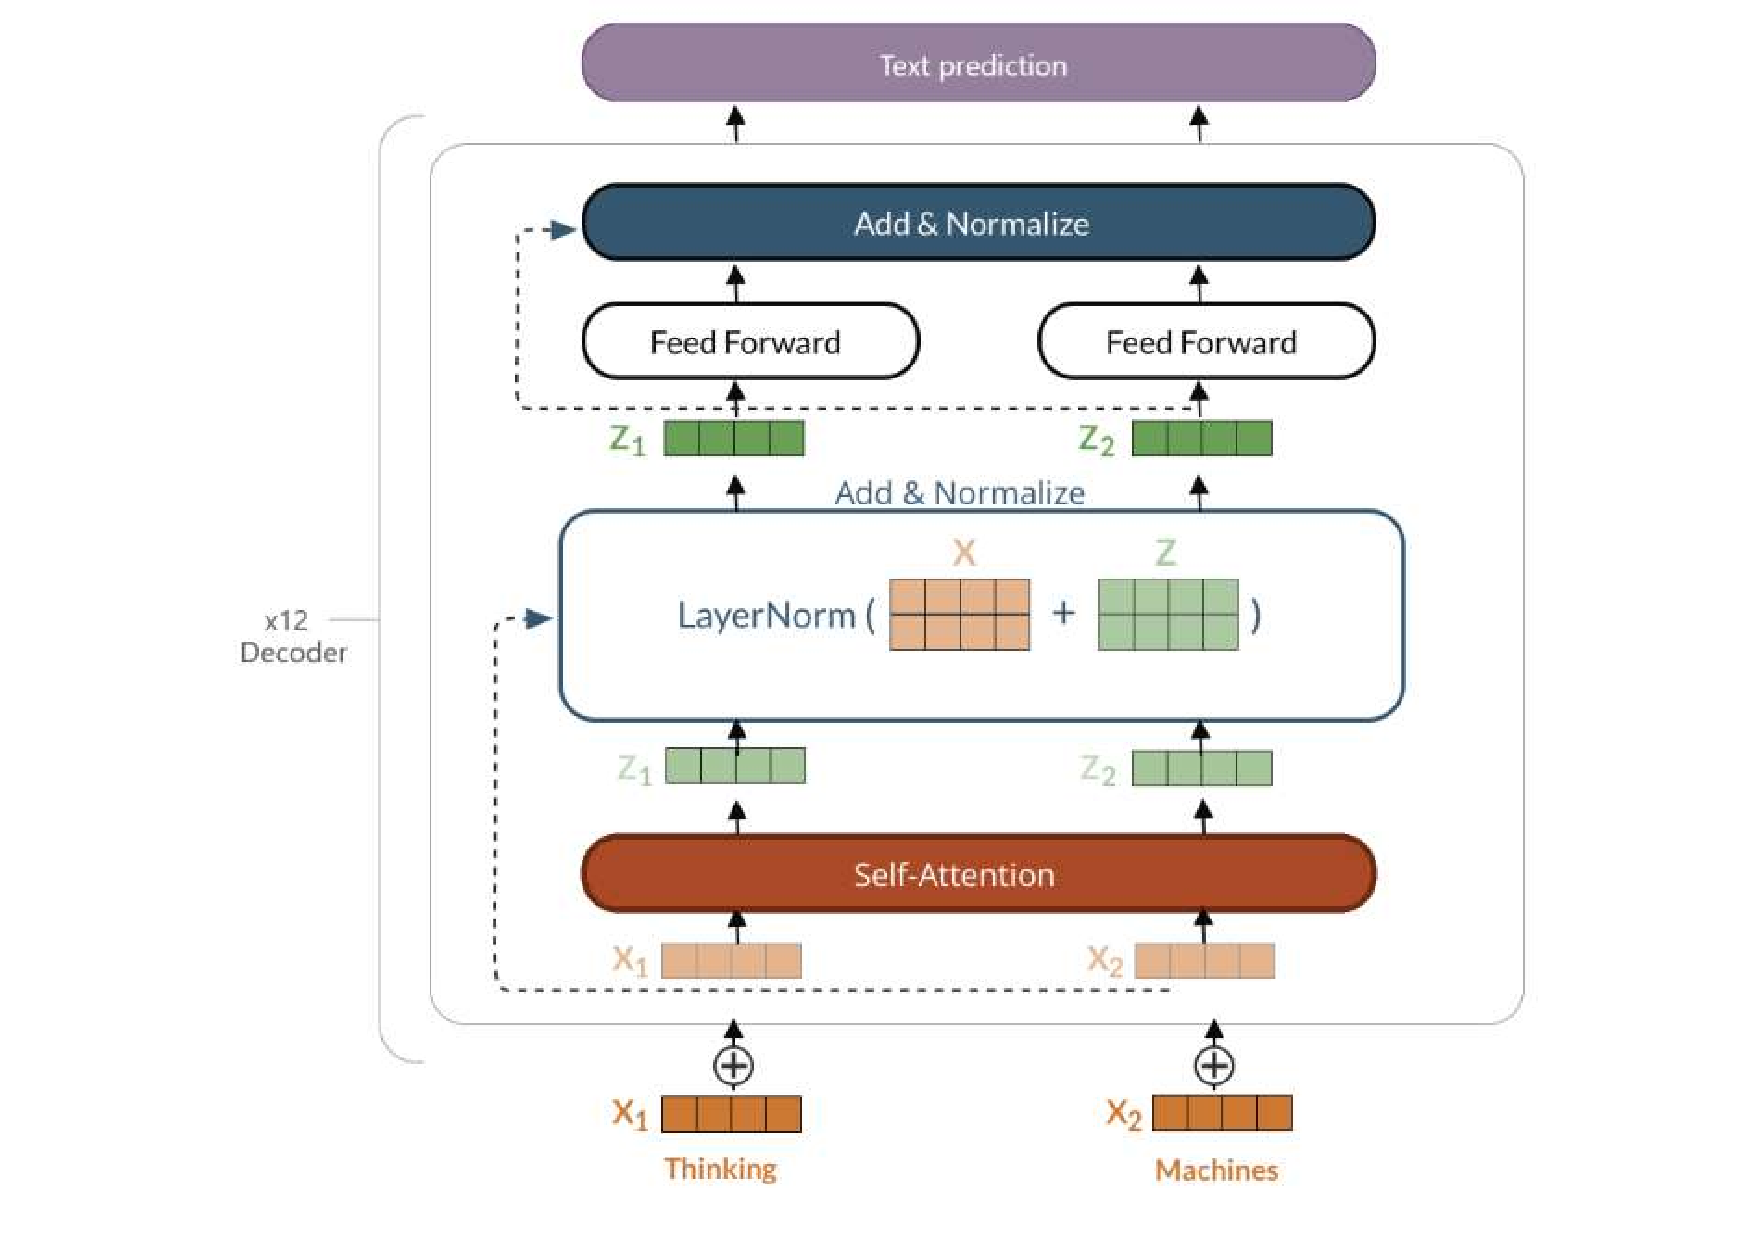
\includegraphics[scale=0.5]{Imagenes/gpt2_architecture}
	\caption{Arquitectura de decodificadores usada por GPT-2} \cite{cristinaalameda}
	\label{fig:gpt2_architecture}
\end{figure}

GPT-2 es un modelo unidireccional que utiliza auto-regresión para generar texto. Se centra en la secuencia anterior a la última palabra y no considera la secuencia posterior. Genera una nueva palabra basada en la secuencia actual y la añade a la entrada para el siguiente paso. Sin embargo, tiene limitaciones, como sesgos en la generación debido al conjunto de datos y al algoritmo de entrenamiento. Además, solo está disponible en inglés, aunque se puede usar Google Translate para otros idiomas. A pesar de esto, los modelos de lenguaje como GPT-2 son útiles para generar texto fluido y completo, prediciendo palabras de un corpus basándose en el contexto anterior.
 
\subsubsection{GPT-3}
GPT-3 aumentó significativamente la cantidad de parámetros en comparación con GPT-2, alcanzando hasta 175 mil millones de parámetros, lo que permitió una mayor complejidad y capacidad de aprendizaje. Debido a su mayor capacidad y tamaño de conjunto de datos, GPT-3 demostró una mejor capacidad para generalizar y comprender una variedad más amplia de contextos y tareas. Además, requiere menos entrenamiento adicional para tareas específicas en comparación con GPT-2.

Por otro lado, y a pesar de la mayor capacidad, GPT-3 logró reducir la generación de texto tóxico en comparación con GPT-2, aunque aún se requirieron estrategias de mitigación.

GPT-3 produjo textos con una mayor precisión y coherencia, lo que resultó en una calidad general de generación de texto más alta y una capacidad para realizar tareas más complejas.
\subsubsection{GPT-4}
GPT-4 según el informe técnico publicado por la propia compañía \citep{GPT4}, es el siguiente modelo de gran escala de OpenAI capaz de aceptar entradas de imagen y texto y producir salidas de texto. Aunque menos capaz que los humanos en muchos escenarios del mundo real, GPT-4 exhibe un rendimiento a nivel humano en diversos puntos de referencia profesionales y académicos, incluida la aprobación de un examen simulado de abogacía con una puntuación alrededor del 10$\%$ superior de los examinados. GPT-4 es un modelo basado en $Transformer$ \ref{sec:Transformers} preentrenado para predecir el siguiente token en un documento. El proceso de alineación posterior al entrenamiento resulta en un mejor rendimiento en medidas de factualidad y adherencia al comportamiento deseado.

Una de las características principales de GPT-4 es su capacidad para procesar entradas de texto y de imagen y producir salidas de texto. Se evaluó en una variedad de exámenes diseñados originalmente para humanos, donde obtuvo resultados destacados, superando en muchos casos a la mayoría de los examinados humanos. Por ejemplo, en un examen simulado de abogacía, GPT-4 obtiene una puntuación que se encuentra en el 10$\%$ superior de los examinados, en contraste con GPT-3.5, que se encuentra en el 1$\%$ inferior.

En una serie de benchmarks tradicionales de NLP, GPT-4 supera tanto a modelos de lenguaje grandes anteriores como a la mayoría de los sistemas de vanguardia (que a menudo tienen entrenamiento específico para el benchmark o ingeniería manual). En el benchmark MMLU, que cubre 57 temas en inglés, GPT-4 no solo supera a los modelos existentes en inglés, sino que también demuestra un rendimiento sólido en otros idiomas.

A pesar de sus capacidades, GPT-4 tiene limitaciones similares a modelos anteriores, como la falta de fiabilidad completa, una ventana de contexto limitada y la incapacidad de aprender de la experiencia. Se debe tener cuidado al usar las salidas de GPT-4, especialmente en contextos donde la fiabilidad es importante. Las capacidades y limitaciones de GPT-4 plantean desafíos de seguridad significativos y novedosos, y se considera que el estudio cuidadoso de estos desafíos es un área de investigación importante dada la posible repercusión societal.
\subsection{Llama}
A diferencia de la creencia común de que más parámetros conducen a un mejor rendimiento, investigaciones recientes muestran que modelos más pequeños entrenados con más datos pueden superar a los modelos más grandes. Se ha desarrollado una serie de modelos llamados LLaMA, \cite{touvron2023llama} que van desde 7B hasta 65B de parámetros, con un rendimiento competitivo en comparación con los mejores LLMs existentes.

Por ejemplo, LLaMA-13B supera a GPT-3 en la mayoría de las pruebas, a pesar de ser 10 veces más pequeño. Se espera que estos modelos democratizen el acceso y el estudio de los LLMs, ya que pueden ejecutarse en una sola GPU. Además, se asegura la compatibilidad con la fuente abierta al utilizar solo datos públicamente disponibles, a diferencia de otros modelos que dependen de datos no disponibles públicamente. El trabajo detalla las modificaciones realizadas en la arquitectura del $transformers$ \ref{sec:Transformers} y el método de entrenamiento, además de presentar el rendimiento de los modelos en comparación con otros LLMs en una serie de pruebas estándar. También se examinan los sesgos y la toxicidad codificados en los modelos, utilizando benchmarks de la comunidad de inteligencia artificial responsable.

El conjunto de datos de entrenamiento es una mezcla de varias fuentes, que cubren un conjunto diverso de dominios. Mayormente reutiliza fuentes de datos que se han utilizado para entrenar otros LLMs, con la restricción de utilizar solo datos públicamente disponibles y compatibles con la distribución abierta.

La tokenización de los datos se lleva a cabo con el algoritmo de codificación de bytes (BPE), utilizando la implementación de  $SentencePiece$ \footnote{El algoritmo $SentencePiece$ \cite{kudo2018sentencepiece} utiliza un enfoque basado en subpalabras, donde construye un vocabulario de subpalabras que se adaptan a la frecuencia de aparición en el corpus de entrenamiento. } . Dividimos todos los números en dígitos individuales y recurrimos a bytes para descomponer caracteres UTF-8 desconocidos. El tamaño total de nuestro conjunto de datos de entrenamiento contiene aproximadamente 1.4T de tokens después de la tokenización. La mayoría de los datos de entrenamiento se utilizan solo una vez durante el entrenamiento, con la excepción de los dominios de Wikipedia y Libros, sobre los cuales se realizan aproximadamente en dos épocas.
\subsection{LaMDA}
\label{sec:LaMDA}
LaMDA, \textit{Language Model for Dialogue Applications} (Modelo de Lenguaje para Aplicaciones de Diálogo), es una familia de modelos de lenguaje neuronal conversacional desarrollados por Google.

La primera generación se anunció en la Google I/O \footnote{Google I/O es una conferencia anual de desarrolladores realizada por Google en Mountain View, California} de 2021 y fue presentada como un modelo de lenguaje conversacional. La segunda generación, presentada en el evento del año siguiente, introdujo mejoras y nuevas capacidades, como la generación de conversaciones originales sobre temas no enseñados previamente. 

LaMDA llamó la atención cuando el ingeniero de Google, Blake Lemoine, afirmó que el chatbot se había vuelto sensible, lo que generó debates sobre la eficacia de la prueba de Turing para determinar la inteligencia artificial general.

Las habilidades conversacionales de LaMDA tardaron años en desarrollarse. Como muchos modelos de lenguaje recientes, incluidos BERT y GPT-3, se basa en $Transformer$ \ref{sec:Transformers}. Esa arquitectura produce un modelo que se puede entrenar para leer muchas palabras (una oración o párrafo, por ejemplo), preste atención a cómo esas palabras se relacionan entre sí y luego prediga qué palabras cree que vendrán a continuación. 

Pero a diferencia de la mayoría de los otros modelos de lenguaje, LaMDA fue entrenado en diálogo. Durante su formación, captó varios de los matices que distinguen la conversación abierta de otras formas de lenguaje. Uno de esos matices es la sensatez. 

El modelo de Transformer que utiliza LaMDA es de solo decodificador y está pre-entrenado en un corpus de texto que incluye documentos y diálogos. Se entrenó con datos de ajuste fino y se probó en diferentes modelos con diferentes hiperparámetros, demostrando superar las respuestas humanas en áreas específicas.

\section{Alucinaciones}
En el campo de la inteligencia artificial (IA), se utiliza el término ``alucinación'' o ``alucinación artificiaL'' para describir respuestas de IA que no parecen estar justificadas por los datos de entrenamiento \cite{edwards2023chatgpt}. Este fenómeno, también conocido como confabulación o delirio, se refiere a la generación de respuestas o creencias que carecen de base sólida \cite{ji2022survey}. Por ejemplo, un chatbot alucinado podría ofrecer información falsa, como afirmar que los ingresos de Tesla fueron de 13.600 millones de dólares, un número aparentemente inventado \cite{lin2022trick}. Otros ejemplos de alucinaciones serían la generación respuestas inventadas como se puede ver en la imagen \ref{img:alucinacion}, donde ChatGPT genera un resumen de un artículo que no existe, o la adición de elementos en el estudio de imágenes, como se ve en la figura\ref{img:alucinacion2}.

\begin{figure}[h]
	\centering
	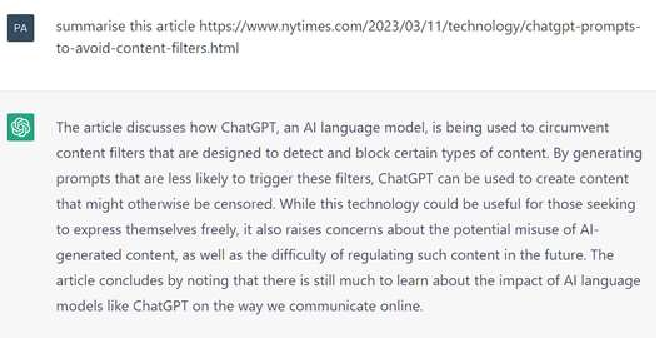
\includegraphics[scale=1]{Imagenes/ejemploAlucinacionGPT}
	\caption{Ejemplo de alucinación de ChatGPT \cite{wikialucinacion}}
	\label{img:alucinacion}
\end{figure}

\begin{figure}[h]
	\centering
	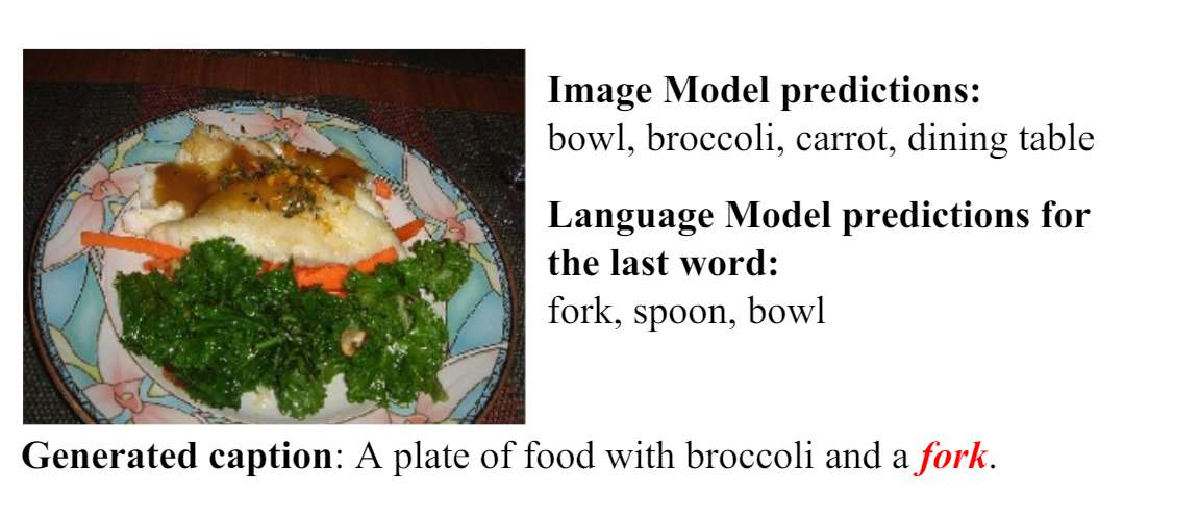
\includegraphics[scale=0.6]{Imagenes/alucinacionImagenes}
	\caption{Ejemplo de alucinación en una imagen \cite{rohrbach2023object}}
	\label{img:alucinacion2}
\end{figure}
Es importante destacar que, aunque se usa el término ``alucinación'' por analogía con la psicología humana, la diferencia fundamental radica en que las alucinaciones de IA se relacionan con respuestas injustificadas más que con percepciones falsas. Algunos investigadores señalan que este término antropomorfiza de manera poco razonable a los ordenadores.

El problema de las alucinaciones de IA se volvió prominente alrededor de 2022 con la introducción de modelos grandes de lenguaje como ChatGPT \cite{zhuo2023exploring}. Los usuarios expresaron preocupación por la capacidad de estos bots para insertar falsedades aparentemente plausibles en sus respuestas. En 2023, los analistas reconocieron las alucinaciones frecuentes como un desafío significativo en la tecnología de modelos de lenguaje \cite{leswing2023microsoft}.

Se cuestiona la confiabilidad del contenido generado por inteligencia artificial en el ámbito científico \cite{machinmastromatteo2023implicaciones}. Según Spinak (2023), los modelos de lenguaje de IA pueden percibir patrones que son imperceptibles para los humanos, lo que resulta en resultados inesperados o incorrectos, fenómeno conocido como ``alucinación'' \cite{spinak2023alucinaciones}. Estas alucinaciones pueden llevar a la producción de contenido falso, especialmente fuera de sus dominios específicos o al tratar con temas complejos o ambiguos, lo cual puede ser lingüísticamente plausible pero no científicamente preciso \cite{sage2023chatgpt}.

\section{Otros trabajos relacionados}
\subsection{Proyecto Cantor}
El proyecto CANTOR (Composición automática de narrativas personales como apoyo a terapia ocupacional basada en reminiscencia) en el que se enmarca este trabajo, desarrolla herramientas digitales utilizando tecnologías de Inteligencia Artificial para construir automáticamente historias de vida que puedan ser reexaminadas posteriormente como apoyo a las terapias ocupacionales de pacientes con demencias.

CANTOR está financiado por el Ministerio de Ciencia e Innovación, en colaboración entre académicos de la Universidad Complutense de Madrid y la Universidad de La Coruña. El objetivo de CANTOR es desarrollar herramientas que faciliten la terapia ocupacional basada en reminiscencia para mejorar la calidad de vida de pacientes con deterioro cognitivo.

En este ámbito se han elaborado varios Trabajos de Fin de Grado en la Facultad de Informática de la UCM. Paso a referir algunos de ellos relacionados con este trabajo. 

\subsubsection{Generación de historias de vida usando técnias de Deep Learning}
\label{sec:trabajocristina}
En el curso 2021-2022, la compañera María Cristina Alameda Salas \cite{cristinaalameda}, en su trabajo de fin de grado, Generación de historias de vida
usando técnicas de Deep Learning, desarrolló un sistema basados en técnicas
de Deep Learning que de soporte a la generación de historias de vida. Partiendo de unos datos de entrada en forma de datos estructurados de tipo biográfico, ese trabajo permite la construcción de un sistema de generación de lenguaje natural, transformador de los datos de entrada a un escrito fluido y coherente, que abarque la representación de los datos de partida de manera completa, sin incorrecciones y lo más cercana posible a una redacción humana. Nuestro objetivo ahora sería el desarrollo de un programa que interactuara con el usuario y nos permitiera obtener toda esa información bibliográfica que da lugar a las historias de vida. 
\subsubsection{Extracción de preguntas a partir de imágenes para personas con problemas de memoria mediante técnicas de Deep Learning}

En 2021, en la UCM se desarrollo un trabajo de extracción de preguntas a partir de imagenes con técnicas de Deep Learning \cite{boto2021extraccion}. Este proyecto ayuda a las personas con problemas de memoria a recordar aspectos de su vida utilizando técnicas de IA como redes convolucionales y recurrentes. Para lograrlo se desarrolló un sistema capaz de extraer preguntas de fotografías que puedan representar recuerdos para las personas con problemas de memoria utilizando un bot que simula una sesión de terapia de reminiscencia.
El usuario ha de enviar fotografías al bot y este se encargará de enviarle, una a una, las preguntas generadas por la red neuronal. En este momento, el usuario deberá recordar todo lo posible sobre la imagen para poder responder a las preguntas y conseguir ejercitar su memoria.

\subsubsection{Extracción de información personal a partir de redes sociales para la creación de un libro de vida}
Este proyecto, desarrollado por \cite{aguilera2021extraccion}, tiene como objetivo principal ayudar a terapeutas ocupacionales en el tratamiento de pacientes con problemas de memoria, especialmente aquellos relacionados con el deterioro cognitivo asociado con la edad. Se propone la creación de una herramienta para desarrollar un libro de vida, una técnica terapéutica conocida como terapia basada en reminiscencia. 

La herramienta combina técnicas de extracción y tratamiento de datos de diferentes redes sociales proporcionadas por el paciente, almacenándolos en una base de datos SQL para obtener la información más relevante. Esta información se utilizará para crear el libro de vida, que se presentará en una interfaz web desarrollada con React. La interfaz permitirá visualizar fácilmente los datos recopilados, utilizando tablas, mapas, líneas de tiempo y galerías de fotos.

\subsubsection{Generación de historias a partir de una base de conocimiento}
En este proyecto, desarrollado por \cite{lucia_latorre_magaz}, se construyó una aplicación para crear relaciones entre palabras e imágenes,
partiendo de unas palabras determinadas. Con las relaciones establecidas la aplicación genera estadísticas a través de las cuales puede evaluarse el progreso del paciente. En cada sesión se trata un tema concreto, pudiéndose elegir el tipo de sesión entre Sesión palabras (se elige una categoría de palabras), Sesión Progreso (se visualiza el avance del paciente a través de estadísticas agrupadas por categorías) o Sesión imágenes (donde se asocia una imagen a un concepto y una categoría).
\subsubsection{Recuerdame 1.0}
Recuerdame 2.0 \cite{recuerdame1.0} presenta la creación de una aplicación que facilite a los terapeutas la realización de terapias basadas en reminiscencia para tratar a pacientes con alzheimer, haciéndolas más ágiles y rápidas.

La aplicación creada es una aplicación web responsive, con una estructura Modelo Vista Controlador creada mediante lenguajes como HTML, CSS, PHP, JavaScript. La aplicación tiene una usabilidad aceptable, pero tiene detalles que mejorar y algunas funcionalidades que no pudieron ser desarrolladas por la falta de tiempo. 

\subsubsection{Recuerdame 2.0}
Durante el curso 2022-2023, la aplicación recuerdame 1.0 fue mejorada dando lugar a recuerdame 2.0 \cite{recuerdame2.0}, para ofrecer una experiencia terapéutica más enriquecedora a pacientes con problemas de memoria. Las mejoras incluyeron la optimización basada en la retroalimentación de usuarios finales, la narración mejorada de Historias de Vida, la generación automática de resúmenes, la integración de terapia con un bot, la mensajería entre terapeutas y cuidadores, y la capacidad de generar vídeos de Historias de Vida. Además, se realizó una evaluación exhaustiva del sistema en instituciones médicas y residencias de ancianos para validar su eficacia.

\subsection{Celia}

Celia, \footnote{\href{https://www.ambito.com/tecnologia/asi-es-celia-la-inteligencia-artificial-adultos-mayores-que-puede-detectar-indicios-alzheimer-n5921639}{Así es Celia, la inteligencia artificial para adultos mayores que puede detectar indicios de alzheimer}} es un chatbot impulsado por inteligencia artificial (IA) desarrollado por la compañía Atlantic, con el respaldo de la Xunta de Galicia en España. Este chatbot tiene como objetivo acompañar, entretener y brindar asistencia a las personas mayores y dependientes, y se destaca por su capacidad para detectar indicios y patrones de enfermedades neurodegenerativas, como el Alzheimer, mediante el análisis de la voz del usuario.

A diferencia de otros asistentes de conversación como Alexa o Siri, Celia va más allá al utilizar herramientas biométricas para medir y monitorear parámetros indicativos no solo de enfermedades neurológicas, sino también de condiciones emocionales como la ansiedad y la depresión.

Celia está disponible para su uso a través de tres plataformas: WhatsApp, la versión web y una aplicación oficial disponible actualmente solo para dispositivos Android. Los usuarios pueden interactuar con Celia a través de mensajes de texto o de voz, y la instalación es sencilla, lo que permite un acceso rápido y eficiente a este recurso tecnológico.

Una característica destacada de Celia es su capacidad para tomar la iniciativa en las conversaciones y proponer actividades sin necesidad de instrucciones. Además, ofrece la posibilidad de establecer recordatorios para citas médicas o la toma de medicamentos, brindando un apoyo integral en la gestión de la salud de los usuarios.
